

\section{Definition}
	
	Dark silicon refers to unpowered silicon on a chip. It stands at a crossroad of multiple important considerations in computer design, and is caused by a cascade of these considerations exacerbating mutual issues until the downstream effect of dark silicon is reached. 
	Fundamentally, dark silicon is a result of a failure of Moore's Law and its more descriptive cousin, Dennardian Scaling. Moore's Law and Dennardian Scaling (henceforth ML-DS) predicted the pattern of CPU design for approximately 4 decades, where a halving of transistor size resulting in a $\sqrt{2}$ multiplication of clock frequency. This relationship has been overtaken by a choice: linearly increasing CPU performance at the cost of exponentially increasing power density, or a 40\% reduction in power usage with each generation but no more performance increases due to decreases transistor size. Ignoring the latter option, the former option of increasing power density directly causes an increase in heat density.
	
	Coupled with the breakdown of ML-DS come limitations in thermal management technology. These coincide to create a circumstance where a chip clocked at its maximum frequency produces more heat than current thermal management methods can handle. This amount of heat results in a decreased life span for the chip, and resulting in a stand-off: run a chip at its maximum throughput or run a chip for its maximum lifetime, but you can't do both. In this case, the latter option is preferable, as a more sustainable chip is better for both ethical and commercial reasons. This is the tension of dark silicon: we want to increase performance of a chip, but we don't want to decrease the lifespan.
	
	Exacerbating the aforementioned issues are the firmware and software layers stacked on top of the hardware layer problems. Naive resource allocation in these layers increases the burden on the CPU. In order to reduce this burden, sections of the stack that are responsible for resource allocation, such as the task scheduler, need to operate with dark silicon principles baked into their operation. 
 

	\begin{figure}[h]
		\caption{The flowchart of dark silicon \cite{DarkSideOfSilicon}}
		\centering
		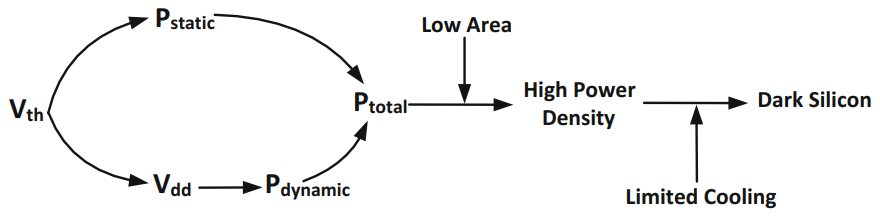
\includegraphics[width=0.7\textwidth]{Dark silicon problem diagram.png}
		\label{Dark silicon problem diagram}
	\end{figure}

	Observing Figure~\ref{Dark silicon problem diagram}, the flowchart of dark silicon can be followed. Condensing power into a smaller area without equivalent advancements in cooling technology results in silicon that can't be safely powered. Dark silicon represents a significant challenge in CPU design, as it broadens the range of considerations that need to be addressed to get maximum performance out of a chip.

\section{Scope}
	\underline{Original Scope:}
	\begin{center}
		\begin{tabular}{|c|c|}
			\hline
			In Scope & Out of Scope\\
			\hline
			Digital Design & Material Design\\
			Task Scheduling Methodologies & Thermal Management\\
			Dynamic Frequency Scaling & Dynamic Voltage Scaling\\
			Memory Driven Computing & Reduced Area Design\\
			Heterogeneous Cores & \\
			\hline
		\end{tabular}
	\end{center}

	Originally, the scope for this project dismissed thermal management from the scope as irrelevant on an FPGA. On reflection, thermal management is a vital inclusion for any investigation of dark silicon methodology.
	
	\vspace{5mm}
	\noindent
	\underline{Revised Scope:}
	\begin{center}
		\begin{tabular}{|c|c|}
			\hline
			In Scope & Out of Scope\\
			\hline
			Digital Design & Material Design\\
			Task Scheduling Methodologies & Dynamic Voltage Scaling\\
			Dynamic Frequency Scaling & Reduced Area Design\\
			Memory Driven Computing & \\
			Heterogeneous Cores & \\
			Thermal Management & \\
			\hline
		\end{tabular}
	\end{center}

	The scope for this project is slightly eclectic. This is a necessity driven by the broad, ranging research space of dark silicon. Solutions to the dark silicon issue are being developed by material scientists, using 3D architectures, photonic interconnects or diamond as a semiconductor instead of silicon. Whilst fascinating, these are all out of scope for a computer and electrical engineering thesis.
	
	Hardware oriented solutions tend to come in the forms of Dynamic Voltage and Frequency Scaling. In scope for this is Dynamic Frequency Scaling (DFS), however dynamic voltage scaling (DVS) is out of scope as it is difficult to implement on an FPGA. Additionally, the hardware oriented approached of heterogeneous cores and memory driven computing are in scope.
	
	Finally, task scheduling methodologies are in scope as resource allocation at an OS level is relevant to optimising CPU utilisation for dark silicon parameters.

